\documentclass[ignorenonframetext,]{beamer}
\setbeamertemplate{caption}[numbered]
\setbeamertemplate{caption label separator}{: }
\setbeamercolor{caption name}{fg=normal text.fg}
\beamertemplatenavigationsymbolsempty
\usepackage{lmodern}
\usepackage{amssymb,amsmath}
\usepackage{ifxetex,ifluatex}
\usepackage{fixltx2e} % provides \textsubscript
\ifnum 0\ifxetex 1\fi\ifluatex 1\fi=0 % if pdftex
  \usepackage[T1]{fontenc}
  \usepackage[utf8]{inputenc}
\else % if luatex or xelatex
  \ifxetex
    \usepackage{mathspec}
  \else
    \usepackage{fontspec}
  \fi
  \defaultfontfeatures{Ligatures=TeX,Scale=MatchLowercase}
\fi
% use upquote if available, for straight quotes in verbatim environments
\IfFileExists{upquote.sty}{\usepackage{upquote}}{}
% use microtype if available
\IfFileExists{microtype.sty}{%
\usepackage{microtype}
\UseMicrotypeSet[protrusion]{basicmath} % disable protrusion for tt fonts
}{}
\newif\ifbibliography
\hypersetup{
            pdftitle={Dealing with complicated data in time series models},
            pdfauthor={Eric Ward},
            pdfborder={0 0 0},
            breaklinks=true}
\urlstyle{same}  % don't use monospace font for urls
\usepackage{color}
\usepackage{fancyvrb}
\newcommand{\VerbBar}{|}
\newcommand{\VERB}{\Verb[commandchars=\\\{\}]}
\DefineVerbatimEnvironment{Highlighting}{Verbatim}{commandchars=\\\{\}}
% Add ',fontsize=\small' for more characters per line
\usepackage{framed}
\definecolor{shadecolor}{RGB}{248,248,248}
\newenvironment{Shaded}{\begin{snugshade}}{\end{snugshade}}
\newcommand{\KeywordTok}[1]{\textcolor[rgb]{0.13,0.29,0.53}{\textbf{#1}}}
\newcommand{\DataTypeTok}[1]{\textcolor[rgb]{0.13,0.29,0.53}{#1}}
\newcommand{\DecValTok}[1]{\textcolor[rgb]{0.00,0.00,0.81}{#1}}
\newcommand{\BaseNTok}[1]{\textcolor[rgb]{0.00,0.00,0.81}{#1}}
\newcommand{\FloatTok}[1]{\textcolor[rgb]{0.00,0.00,0.81}{#1}}
\newcommand{\ConstantTok}[1]{\textcolor[rgb]{0.00,0.00,0.00}{#1}}
\newcommand{\CharTok}[1]{\textcolor[rgb]{0.31,0.60,0.02}{#1}}
\newcommand{\SpecialCharTok}[1]{\textcolor[rgb]{0.00,0.00,0.00}{#1}}
\newcommand{\StringTok}[1]{\textcolor[rgb]{0.31,0.60,0.02}{#1}}
\newcommand{\VerbatimStringTok}[1]{\textcolor[rgb]{0.31,0.60,0.02}{#1}}
\newcommand{\SpecialStringTok}[1]{\textcolor[rgb]{0.31,0.60,0.02}{#1}}
\newcommand{\ImportTok}[1]{#1}
\newcommand{\CommentTok}[1]{\textcolor[rgb]{0.56,0.35,0.01}{\textit{#1}}}
\newcommand{\DocumentationTok}[1]{\textcolor[rgb]{0.56,0.35,0.01}{\textbf{\textit{#1}}}}
\newcommand{\AnnotationTok}[1]{\textcolor[rgb]{0.56,0.35,0.01}{\textbf{\textit{#1}}}}
\newcommand{\CommentVarTok}[1]{\textcolor[rgb]{0.56,0.35,0.01}{\textbf{\textit{#1}}}}
\newcommand{\OtherTok}[1]{\textcolor[rgb]{0.56,0.35,0.01}{#1}}
\newcommand{\FunctionTok}[1]{\textcolor[rgb]{0.00,0.00,0.00}{#1}}
\newcommand{\VariableTok}[1]{\textcolor[rgb]{0.00,0.00,0.00}{#1}}
\newcommand{\ControlFlowTok}[1]{\textcolor[rgb]{0.13,0.29,0.53}{\textbf{#1}}}
\newcommand{\OperatorTok}[1]{\textcolor[rgb]{0.81,0.36,0.00}{\textbf{#1}}}
\newcommand{\BuiltInTok}[1]{#1}
\newcommand{\ExtensionTok}[1]{#1}
\newcommand{\PreprocessorTok}[1]{\textcolor[rgb]{0.56,0.35,0.01}{\textit{#1}}}
\newcommand{\AttributeTok}[1]{\textcolor[rgb]{0.77,0.63,0.00}{#1}}
\newcommand{\RegionMarkerTok}[1]{#1}
\newcommand{\InformationTok}[1]{\textcolor[rgb]{0.56,0.35,0.01}{\textbf{\textit{#1}}}}
\newcommand{\WarningTok}[1]{\textcolor[rgb]{0.56,0.35,0.01}{\textbf{\textit{#1}}}}
\newcommand{\AlertTok}[1]{\textcolor[rgb]{0.94,0.16,0.16}{#1}}
\newcommand{\ErrorTok}[1]{\textcolor[rgb]{0.64,0.00,0.00}{\textbf{#1}}}
\newcommand{\NormalTok}[1]{#1}

% Prevent slide breaks in the middle of a paragraph:
\widowpenalties 1 10000
\raggedbottom

\AtBeginPart{
  \let\insertpartnumber\relax
  \let\partname\relax
  \frame{\partpage}
}
\AtBeginSection{
  \ifbibliography
  \else
    \let\insertsectionnumber\relax
    \let\sectionname\relax
    \frame{\sectionpage}
  \fi
}
\AtBeginSubsection{
  \let\insertsubsectionnumber\relax
  \let\subsectionname\relax
  \frame{\subsectionpage}
}

\setlength{\parindent}{0pt}
\setlength{\parskip}{6pt plus 2pt minus 1pt}
\setlength{\emergencystretch}{3em}  % prevent overfull lines
\providecommand{\tightlist}{%
  \setlength{\itemsep}{0pt}\setlength{\parskip}{0pt}}
\setcounter{secnumdepth}{0}

\title{Dealing with complicated data in time series models}
\subtitle{FISH 507 -- Applied Time Series Analysis}
\author{Eric Ward}
\date{12 Mar 2019}

\begin{document}
\frame{\titlepage}

\begin{frame}{Modeling zero-inflated data}

Zero-inflated = data with excess of zero counts

The degree of zero-inflation may be extreme

\begin{center}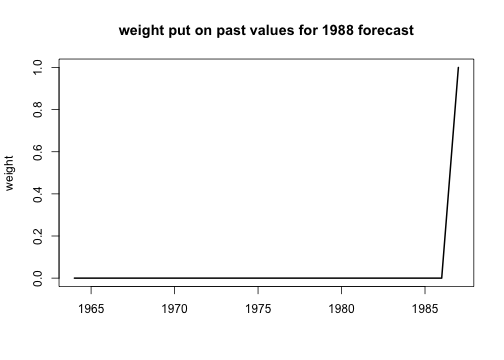
\includegraphics{lec_19_zero-inflated_files/figure-beamer/unnamed-chunk-1-1} \end{center}

\end{frame}

\begin{frame}{Modeling zero-inflated data}

Zero-inflated = data with excess of zero counts

Or more subtle

\begin{center}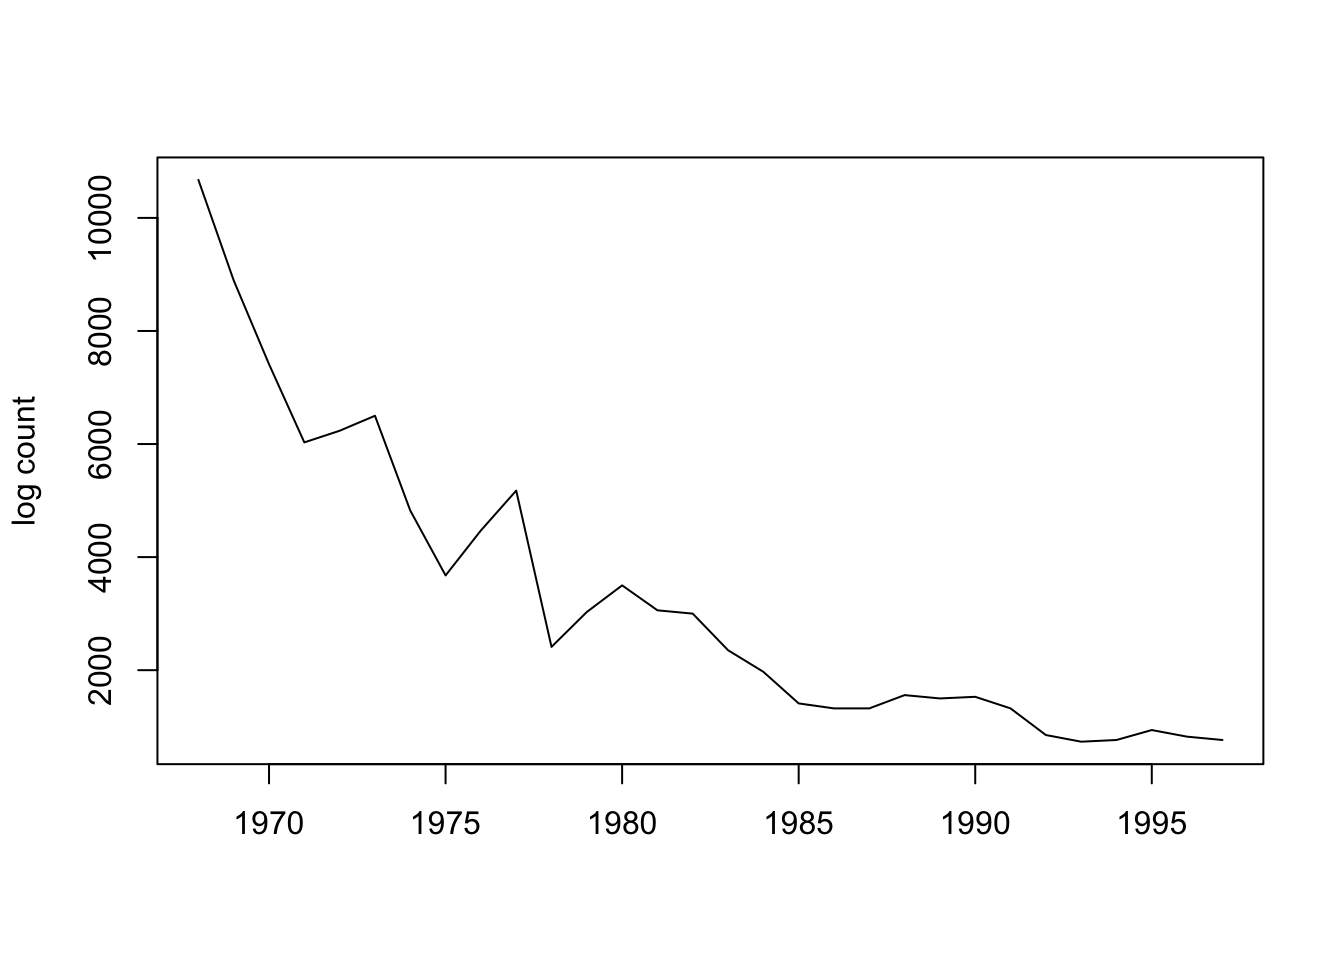
\includegraphics{lec_19_zero-inflated_files/figure-beamer/unnamed-chunk-2-1} \end{center}

\end{frame}

\begin{frame}{Lots of options for dealing with zeros}

\begin{enumerate}
\def\labelenumi{\arabic{enumi}.}
\item
  Remove them from the dataset and ignore them
\item
  Transform your data
\item
  Work with complicated statistical models
\end{enumerate}

\end{frame}

\begin{frame}{1. Dropping zeros}

\begin{center}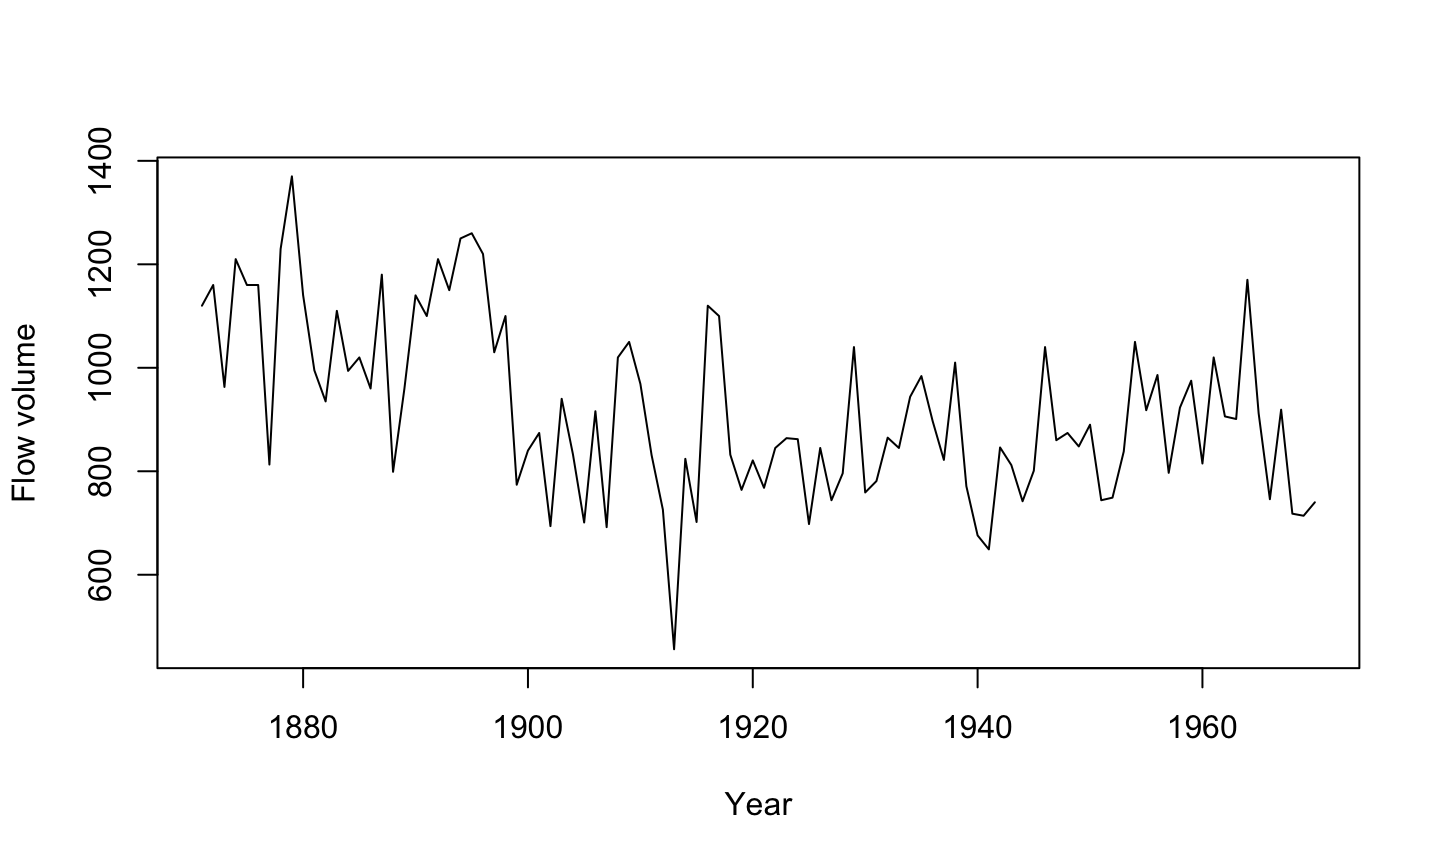
\includegraphics{lec_19_zero-inflated_files/figure-beamer/unnamed-chunk-3-1} \end{center}

\end{frame}

\begin{frame}{1. Dropping zeros}

\begin{center}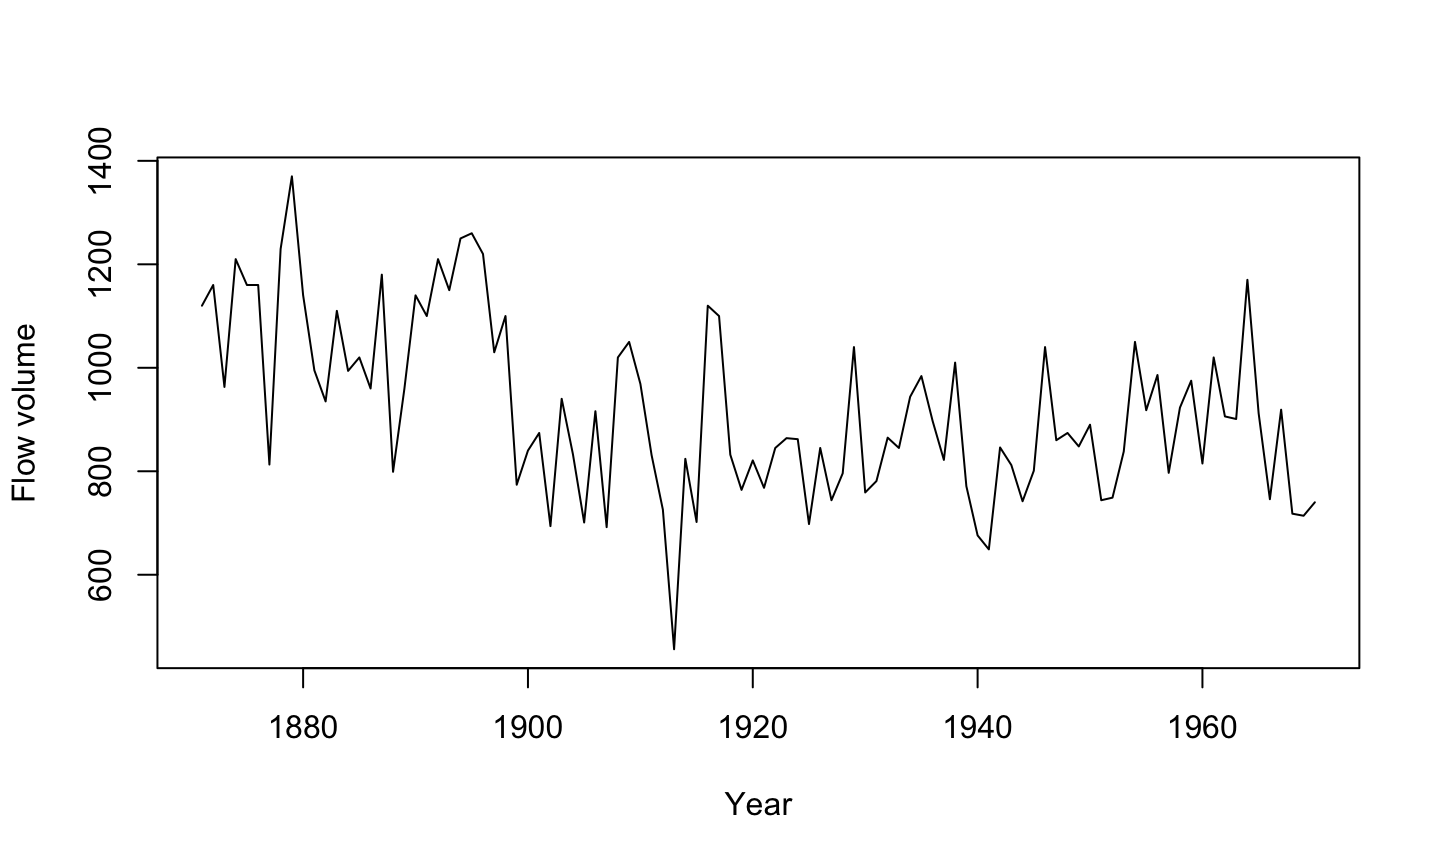
\includegraphics{lec_19_zero-inflated_files/figure-beamer/unnamed-chunk-4-1} \end{center}

\end{frame}

\begin{frame}{1. Dropping zeros}

Can work in a limited number of cases BUT

Becomes problematic for

\begin{itemize}
\item
  models that depend on autoregressive structure
\item
  models that don't allow for missing data / NAs
\item
  datasets where the zeros aren't random (Daphnia example)
\item
  zeros are caused by response (density dependence, etc)
\end{itemize}

\end{frame}

\begin{frame}{2. Transforming data}

With zero-inflated data, it's common to add a small number and transform
the results -- ln(), sqrt(), etc.

\begin{itemize}
\tightlist
\item
  Problem: what constant should be added before we apply the
  transformation?
\end{itemize}

\end{frame}

\begin{frame}{Example: Lake WA Conochilus}

\begin{center}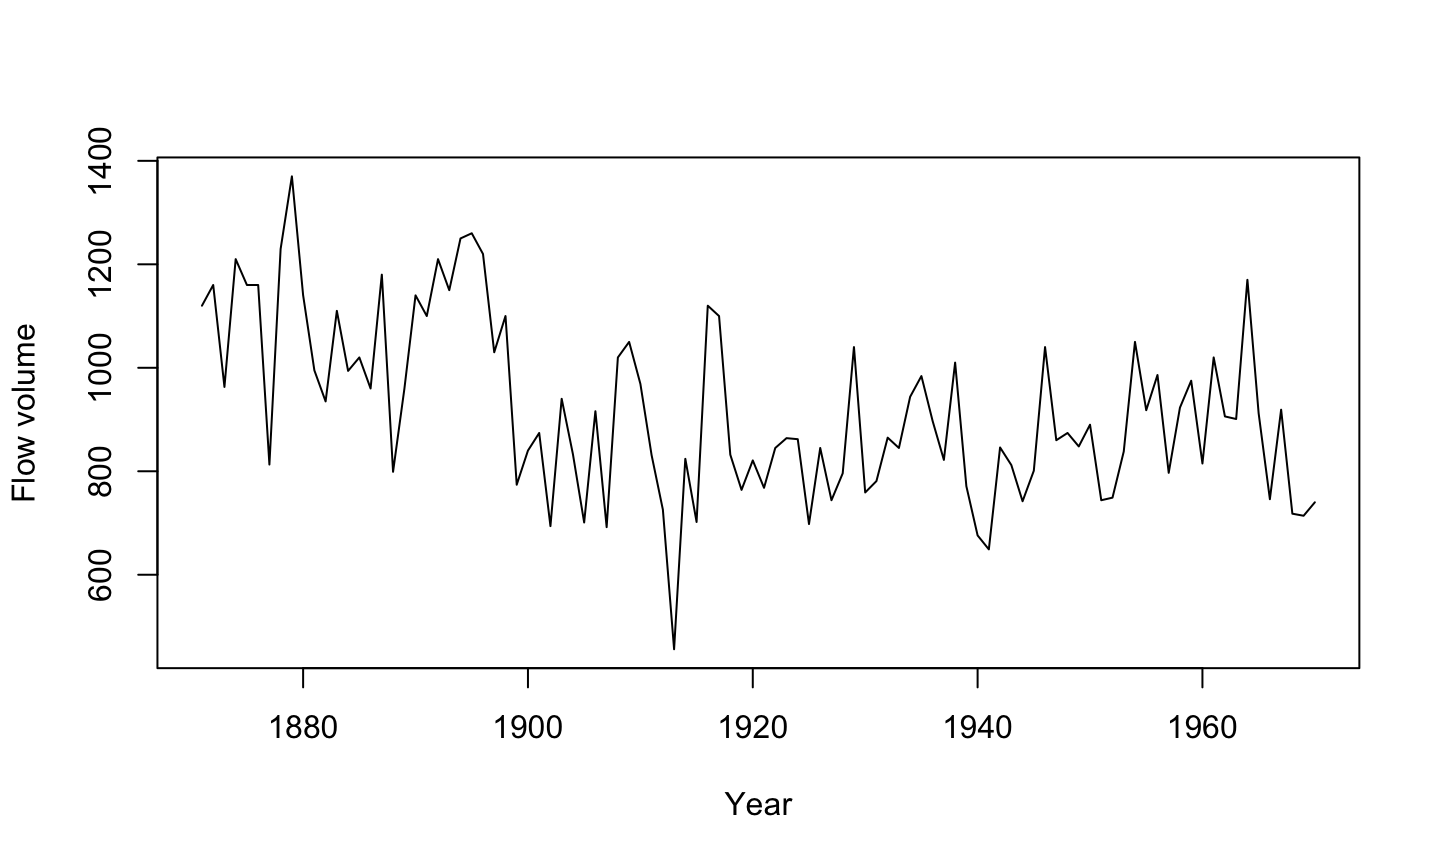
\includegraphics{lec_19_zero-inflated_files/figure-beamer/unnamed-chunk-5-1} \end{center}

\end{frame}

\begin{frame}{Example: Lake WA Conochilus}

\begin{center}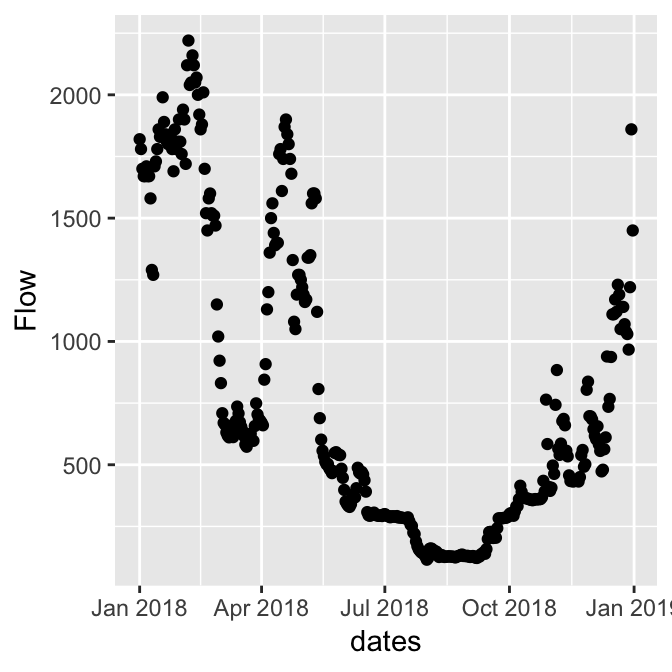
\includegraphics{lec_19_zero-inflated_files/figure-beamer/unnamed-chunk-6-1} \end{center}

\end{frame}

\begin{frame}{Example: Lake WA Conochilus}

Lots of problems with this approach generally

\begin{itemize}
\item
  choice of constant is subjective
\item
  leads to biases in parameters being estimated
\end{itemize}

Example: let's fit auto.arima() to this time series using different
constants

\end{frame}

\begin{frame}{Example: Lake WA Conochilus}

log(Conochilus + 0.001) = ARIMA(3,1,1) + no drift

log(Conochilus + 0.01) = ARIMA(3,1,2) + no drift

log(Conochilus + 0.1) = ARIMA(2,1,1) + no drift

log(Conochilus + 1) = ARIMA(5,1,0) + drift

\end{frame}

\begin{frame}{References for adding constants (or not)}

Ekwaru et al. 2017
\href{https://amstat.tandfonline.com/doi/abs/10.1080/19466315.2017.1369900?journalCode=usbr20\#.XIe-RBNKiM4}{link}

O'hara and Kotze 2010
\href{https://besjournals.onlinelibrary.wiley.com/doi/full/10.1111/j.2041-210X.2010.00021.x}{link}

\end{frame}

\begin{frame}{3. Using more complicated statistical models}

\begin{enumerate}
\def\labelenumi{\arabic{enumi}.}
\item
  Tweedie distribution
\item
  Delta or hurdle- models
\end{enumerate}

\end{frame}

\begin{frame}{Tweedie distribution}

\begin{itemize}
\item
  Tweedie is very flexible
\item
  Skewed continuous distribution with point mass at zero

  \begin{itemize}
  \tightlist
  \item
    unlike Gamma, which is undefined at zero
  \end{itemize}
\end{itemize}

\end{frame}

\begin{frame}{Implementation in R}

Lots of existing family support

\begin{itemize}
\tightlist
\item
  Specify link function (\emph{q}) - related predicted values to
  covariates
\end{itemize}

\(μ_i^q = x_i^Tb\)

\begin{itemize}
\tightlist
\item
  Specify power function (\emph{p}) - relates variance to mean
\end{itemize}

\(var(y_i) = phi * μ_i^p\)

\begin{itemize}
\tightlist
\item
  When 1 \textless{} \emph{p} \textless{} 2, behavior is compound
  Poisson / Tweedie
\end{itemize}

\end{frame}

\begin{frame}[fragile]{Let's apply GLMs with Tweedie to Lake WA data}

\begin{Shaded}
\begin{Highlighting}[]
\KeywordTok{library}\NormalTok{(statmod)}
\NormalTok{g =}\StringTok{ }\KeywordTok{glm}\NormalTok{(Conochilus }\OperatorTok{~}\StringTok{ }\DecValTok{1}\NormalTok{, }\DataTypeTok{family=}
    \KeywordTok{tweedie}\NormalTok{(}\DataTypeTok{var.power=}\FloatTok{1.3}\NormalTok{,}\DataTypeTok{link.power=}\DecValTok{0}\NormalTok{), }
  \DataTypeTok{data=}\KeywordTok{as.data.frame}\NormalTok{(lakeWAplanktonRaw))}
\end{Highlighting}
\end{Shaded}

\end{frame}

\begin{frame}[fragile]{What's the right variance power to choose?}

Package `tweedie' does ML estimation of the \emph{p} parameter.

\begin{Shaded}
\begin{Highlighting}[]
\KeywordTok{library}\NormalTok{(tweedie)}
\NormalTok{tp =}\StringTok{ }\KeywordTok{tweedie.profile}\NormalTok{(Conochilus }\OperatorTok{~}\StringTok{ }\DecValTok{1}\NormalTok{, }
  \DataTypeTok{p.vec =} \KeywordTok{seq}\NormalTok{(}\DecValTok{1}\NormalTok{,}\DecValTok{2}\NormalTok{,}\DataTypeTok{by=}\FloatTok{0.1}\NormalTok{), }
  \DataTypeTok{data=}\KeywordTok{as.data.frame}\NormalTok{(lakeWAplanktonRaw))}
\end{Highlighting}
\end{Shaded}

\end{frame}

\begin{frame}[fragile]{What's the right variance power to choose?}

\begin{Shaded}
\begin{Highlighting}[]
\KeywordTok{plot}\NormalTok{(tp, }\DataTypeTok{xlab=}\StringTok{"p"}\NormalTok{, }\DataTypeTok{ylab=}\StringTok{"log lik"}\NormalTok{)}
\end{Highlighting}
\end{Shaded}

\begin{center}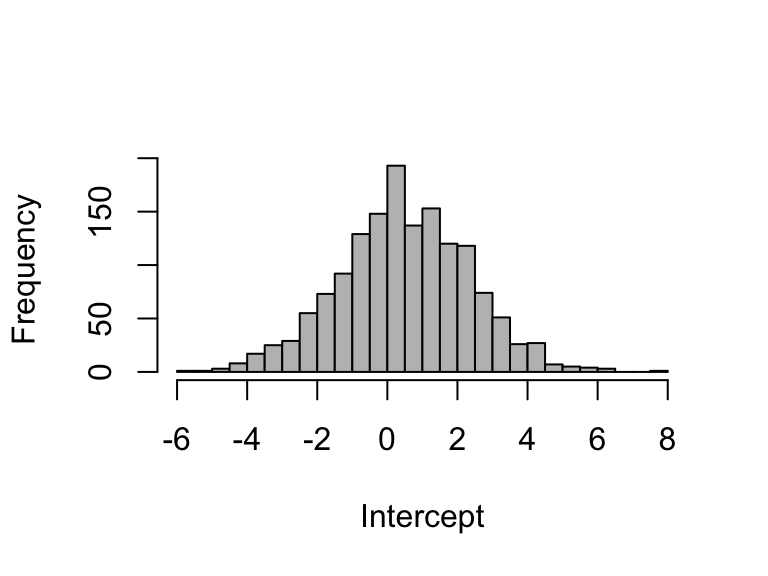
\includegraphics{lec_19_zero-inflated_files/figure-beamer/unnamed-chunk-9-1} \end{center}

\end{frame}

\begin{frame}[fragile]{Other implementations in R}

Also supported in `mgcv'. \emph{p} parameter may be fixed

\begin{Shaded}
\begin{Highlighting}[]
\KeywordTok{gam}\NormalTok{(Conochilus}\OperatorTok{~}\KeywordTok{s}\NormalTok{(year), }\DataTypeTok{family=}\KeywordTok{Tweedie}\NormalTok{(}\FloatTok{1.25}\NormalTok{,}\KeywordTok{power}\NormalTok{(.}\DecValTok{1}\NormalTok{)),}
  \DataTypeTok{data=}\KeywordTok{as.data.frame}\NormalTok{(lakeWAplanktonRaw))}
\end{Highlighting}
\end{Shaded}

or estimated

\begin{Shaded}
\begin{Highlighting}[]
\KeywordTok{gam}\NormalTok{(Conochilus}\OperatorTok{~}\KeywordTok{s}\NormalTok{(year), }\DataTypeTok{family=}\KeywordTok{tw}\NormalTok{(),}
  \DataTypeTok{data=}\KeywordTok{as.data.frame}\NormalTok{(lakeWAplanktonRaw))}
\end{Highlighting}
\end{Shaded}

\end{frame}

\begin{frame}{Delta (aka hurdle models)}

Tweedie models every data point as being generated from the same process

Alternative: use delta- or hurdle- models

\begin{itemize}
\item
  These model the zeros with one sub-model, and the positive values with
  a second sub-model
\item
  Very widely used in fisheries (index standardization etc)
\end{itemize}

\end{frame}

\begin{frame}{Sub-models}

Binomial data (logit link) \(logit(p_i) = log(p_i/(1-p_i)) = BX_i\)

Positive model (log link generally) \(log(u_i) = CZ_i\)

\begin{itemize}
\tightlist
\item
  Poisson, Gamma, NegBinomial, etc
\item
  \(Z_i\) and \(X_i\) may be identical
\item
  Where are the error terms? (GLMMs)
\end{itemize}

\end{frame}

\begin{frame}{Time series}

Adding these error terms allow us to turn conventional GLM into time
series models with autoregressive behavior, e.g.
\[Y_t \sim Bernoulli(p_t)\] \[logit(p_t) = logit(X_t)\]
\[X_{t} = BX_{t-1} + \epsilon_{t-1}\]
\[\epsilon_t \sim Normal(0, \sigma)\]

\begin{itemize}
\tightlist
\item
  Any DLM or SS model can be extended to include non-normal errors
\end{itemize}

\end{frame}

\begin{frame}[fragile]{Hurdle models}

Delta-GLM: We'll start fitting 2 models to the Conochilus data

\begin{Shaded}
\begin{Highlighting}[]
\NormalTok{lakeWAplanktonRaw =}\StringTok{ }\KeywordTok{as.data.frame}\NormalTok{(lakeWAplanktonRaw)}
\NormalTok{lakeWAplanktonRaw}\OperatorTok{$}\NormalTok{present =}\StringTok{ }
\StringTok{  }\KeywordTok{ifelse}\NormalTok{(lakeWAplanktonRaw}\OperatorTok{$}\NormalTok{Conochilus }\OperatorTok{>}\StringTok{ }\DecValTok{0}\NormalTok{, }\DecValTok{1}\NormalTok{, }\DecValTok{0}\NormalTok{)}

\NormalTok{model_}\DecValTok{01}\NormalTok{ =}\StringTok{ }\KeywordTok{glm}\NormalTok{(present }\OperatorTok{~}\StringTok{ }\NormalTok{Year }\OperatorTok{+}\StringTok{ }\KeywordTok{as.factor}\NormalTok{(Month),}
  \DataTypeTok{data=}\NormalTok{lakeWAplanktonRaw, }\DataTypeTok{family =}\NormalTok{ binomial)}
\NormalTok{model_pos =}\StringTok{ }\KeywordTok{glm}\NormalTok{(Conochilus }\OperatorTok{~}\StringTok{ }\NormalTok{Year }\OperatorTok{+}\StringTok{ }\KeywordTok{as.factor}\NormalTok{(Month),}
  \DataTypeTok{data=}\NormalTok{lakeWAplanktonRaw[}\KeywordTok{which}\NormalTok{(lakeWAplanktonRaw}\OperatorTok{$}\NormalTok{Conochilus}\OperatorTok{>}\DecValTok{0}\NormalTok{),],}
  \DataTypeTok{family =} \KeywordTok{Gamma}\NormalTok{(}\DataTypeTok{link=}\StringTok{"log"}\NormalTok{))}
\end{Highlighting}
\end{Shaded}

\end{frame}

\begin{frame}[fragile]{Hurdle models}

Now we can combine predictions from these models for estimates of
Conochilus density

\begin{Shaded}
\begin{Highlighting}[]
\NormalTok{lakeWAplanktonRaw}\OperatorTok{$}\NormalTok{glm_pred =}\StringTok{ }\KeywordTok{predict}\NormalTok{(model_}\DecValTok{01}\NormalTok{, }
  \DataTypeTok{newdata=}\NormalTok{lakeWAplanktonRaw, }\DataTypeTok{type=}\StringTok{"response"}\NormalTok{) }\OperatorTok{*}\StringTok{ }
\StringTok{  }\KeywordTok{predict}\NormalTok{(model_pos, }
  \DataTypeTok{newdata=}\NormalTok{lakeWAplanktonRaw, }\DataTypeTok{type=}\StringTok{"response"}\NormalTok{)}
\end{Highlighting}
\end{Shaded}

\begin{center}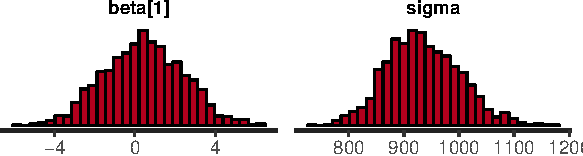
\includegraphics{lec_19_zero-inflated_files/figure-beamer/unnamed-chunk-14-1} \end{center}

\end{frame}

\begin{frame}[fragile]{Hurdle models}

In the last example, we used glm() to put the model pieces together
ourselves.

Alternatives:

\begin{Shaded}
\begin{Highlighting}[]
\NormalTok{pscl}\OperatorTok{::}\KeywordTok{hurdle}\NormalTok{()}
\end{Highlighting}
\end{Shaded}

\end{frame}

\begin{frame}[fragile]{Hurdle models via mgcv}

Given the fits to the hurdle model with GLM() weren't great, it may be
worthwhile to try a GAM

Delta-GAM: We'll start fitting 2 models to the Conochilus data

\begin{Shaded}
\begin{Highlighting}[]
\NormalTok{lakeWAplanktonRaw =}\StringTok{ }\KeywordTok{as.data.frame}\NormalTok{(lakeWAplanktonRaw)}
\NormalTok{lakeWAplanktonRaw}\OperatorTok{$}\NormalTok{present =}\StringTok{ }
\StringTok{  }\KeywordTok{ifelse}\NormalTok{(lakeWAplanktonRaw}\OperatorTok{$}\NormalTok{Conochilus }\OperatorTok{>}\StringTok{ }\DecValTok{0}\NormalTok{, }\DecValTok{1}\NormalTok{, }\DecValTok{0}\NormalTok{)}

\NormalTok{model_}\DecValTok{01}\NormalTok{ =}\StringTok{ }\KeywordTok{gam}\NormalTok{(present }\OperatorTok{~}\StringTok{ }\KeywordTok{s}\NormalTok{(Year) }\OperatorTok{+}\StringTok{ }
\StringTok{    }\KeywordTok{s}\NormalTok{(Month,}\DataTypeTok{bs=}\StringTok{"cc"}\NormalTok{,}\DataTypeTok{k=}\DecValTok{12}\NormalTok{), }
  \DataTypeTok{data=}\NormalTok{lakeWAplanktonRaw, }\DataTypeTok{family =}\NormalTok{ binomial)}
\NormalTok{model_pos =}\StringTok{ }\KeywordTok{gam}\NormalTok{(Conochilus }\OperatorTok{~}\StringTok{ }\KeywordTok{s}\NormalTok{(Year) }\OperatorTok{+}\StringTok{ }
\StringTok{    }\KeywordTok{s}\NormalTok{(Month,}\DataTypeTok{bs=}\StringTok{"cc"}\NormalTok{,}\DataTypeTok{k=}\DecValTok{12}\NormalTok{),}
  \DataTypeTok{data=}\NormalTok{lakeWAplanktonRaw[}\KeywordTok{which}\NormalTok{(lakeWAplanktonRaw}\OperatorTok{$}\NormalTok{Conochilus}\OperatorTok{>}\DecValTok{0}\NormalTok{),], }
  \DataTypeTok{family =} \KeywordTok{Gamma}\NormalTok{(}\DataTypeTok{link=}\StringTok{"log"}\NormalTok{))}
\end{Highlighting}
\end{Shaded}

\end{frame}

\begin{frame}[fragile]{Hurdle models}

Predictions via the GAM. These look maybe slightly better but don't
appear to capture really high observations

\begin{Shaded}
\begin{Highlighting}[]
\NormalTok{lakeWAplanktonRaw}\OperatorTok{$}\NormalTok{gam_pred =}\StringTok{ }\KeywordTok{predict}\NormalTok{(model_}\DecValTok{01}\NormalTok{, }
  \DataTypeTok{newdata=}\NormalTok{lakeWAplanktonRaw, }\DataTypeTok{type=}\StringTok{"response"}\NormalTok{) }\OperatorTok{*}\StringTok{ }
\StringTok{  }\KeywordTok{predict}\NormalTok{(model_pos, }
  \DataTypeTok{newdata=}\NormalTok{lakeWAplanktonRaw, }\DataTypeTok{type=}\StringTok{"response"}\NormalTok{)}
\end{Highlighting}
\end{Shaded}

\begin{center}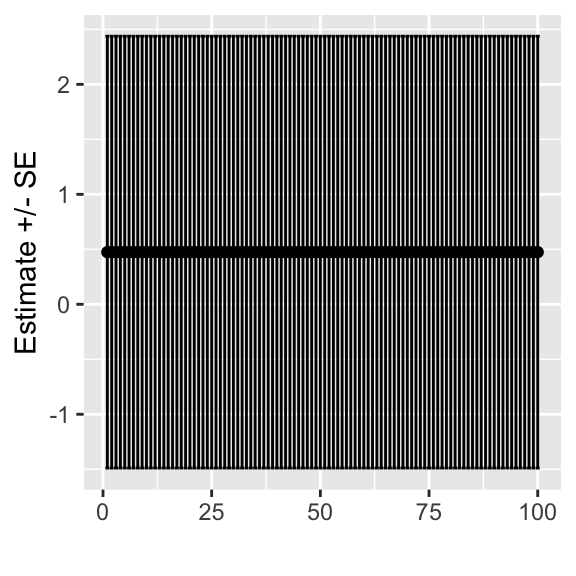
\includegraphics{lec_19_zero-inflated_files/figure-beamer/unnamed-chunk-18-1} \end{center}

\end{frame}

\begin{frame}[fragile]{Extensions with adding mixed effects}

Several R packages out there. `glmmTMB' makes ML estimation relatively
straightforward if your hurdle model = Poisson or NegBin.

\begin{itemize}
\tightlist
\item
  Instead we'll add mixed effects with the Tweedie
\end{itemize}

\begin{Shaded}
\begin{Highlighting}[]
\NormalTok{mod <-}\StringTok{ }\KeywordTok{glmmTMB}\NormalTok{(Conochilus}\OperatorTok{~}\KeywordTok{as.factor}\NormalTok{(Month) }\OperatorTok{+}\StringTok{ }\NormalTok{(}\DecValTok{1}\OperatorTok{|}\NormalTok{Year), }
  \DataTypeTok{family=}\KeywordTok{tweedie}\NormalTok{(), lakeWAplanktonRaw)}
\end{Highlighting}
\end{Shaded}

\end{frame}

\begin{frame}{Extensions with adding mixed effects}

Comparing these models so far,

\begin{tabular}{l|l}
\hline
Model & Cor (pred,obs)\\
\hline
GLM & 0.355\\
\hline
GAM & 0.377\\
\hline
GLMM & 0.339\\
\hline
\end{tabular}

\end{frame}

\begin{frame}[fragile]{brms}

Bayesian hurdle models, optionally with smooth functions and random
effects!

Start with month (factor) and Year (linear trend) in positive model,
hurdle is intercept only

\begin{Shaded}
\begin{Highlighting}[]
\KeywordTok{library}\NormalTok{(brms)}
\NormalTok{mod =}\StringTok{ }\KeywordTok{brm}\NormalTok{(}\KeywordTok{bf}\NormalTok{(Conochilus}\OperatorTok{~}\StringTok{ }\KeywordTok{as.factor}\NormalTok{(Month) }\OperatorTok{+}\StringTok{ }\NormalTok{Year, }
\NormalTok{       hu }\OperatorTok{~}\StringTok{ }\DecValTok{1}\NormalTok{, }
      \DataTypeTok{data =}\NormalTok{ lakeWAplanktonRaw, }\DataTypeTok{family =} \KeywordTok{hurdle_gamma}\NormalTok{(), }
        \DataTypeTok{chains=}\DecValTok{1}\NormalTok{, }\DataTypeTok{iter=}\DecValTok{1000}\NormalTok{)}
\end{Highlighting}
\end{Shaded}

\end{frame}

\begin{frame}[fragile]{brms}

Now we can add month covariates to the hurdle part, and a smooth
function on Year

\begin{itemize}
\tightlist
\item
  We use \emph{k} to select the wiggliness of the smooth.
\item
  It can be selected automatically, but probably better to put some
  thought into this!
\end{itemize}

\begin{Shaded}
\begin{Highlighting}[]
\KeywordTok{library}\NormalTok{(brms)}
\NormalTok{mod =}\StringTok{ }\KeywordTok{brm}\NormalTok{(}\KeywordTok{bf}\NormalTok{(Conochilus}\OperatorTok{~}\StringTok{ }\KeywordTok{as.factor}\NormalTok{(Month) }\OperatorTok{+}\StringTok{ }\KeywordTok{s}\NormalTok{(Year, }\DataTypeTok{k=}\DecValTok{10}\NormalTok{), }
\NormalTok{       hu }\OperatorTok{~}\StringTok{ }\KeywordTok{as.factor}\NormalTok{(Month), }
      \DataTypeTok{data =}\NormalTok{ lakeWAplanktonRaw, }\DataTypeTok{family =} \KeywordTok{hurdle_gamma}\NormalTok{(), }
        \DataTypeTok{chains=}\DecValTok{1}\NormalTok{, }\DataTypeTok{iter=}\DecValTok{1000}\NormalTok{)}
\end{Highlighting}
\end{Shaded}

\end{frame}

\begin{frame}[fragile]{brms}

Or we could include the month term as a random effect (intercept)

\begin{Shaded}
\begin{Highlighting}[]
\KeywordTok{library}\NormalTok{(brms)}
\NormalTok{mod =}\StringTok{ }\KeywordTok{brm}\NormalTok{(}\KeywordTok{bf}\NormalTok{(Conochilus}\OperatorTok{~}\StringTok{ }\KeywordTok{as.factor}\NormalTok{(Month) }\OperatorTok{+}\StringTok{ }\KeywordTok{s}\NormalTok{(Year, }\DataTypeTok{k=}\DecValTok{10}\NormalTok{), }
\NormalTok{       hu }\OperatorTok{~}\StringTok{ }\KeywordTok{as.factor}\NormalTok{(Month), }
      \DataTypeTok{data =}\NormalTok{ lakeWAplanktonRaw, }\DataTypeTok{family =} \KeywordTok{hurdle_gamma}\NormalTok{(), }
        \DataTypeTok{chains=}\DecValTok{1}\NormalTok{, }\DataTypeTok{iter=}\DecValTok{1000}\NormalTok{)}
\end{Highlighting}
\end{Shaded}

\end{frame}

\begin{frame}[fragile]{brms}

Each of these models can be evaluated with LOOIC for model selection,
e.g.

\begin{Shaded}
\begin{Highlighting}[]
\KeywordTok{library}\NormalTok{(brms)}
\NormalTok{mod =}\StringTok{ }\KeywordTok{brm}\NormalTok{(}\KeywordTok{bf}\NormalTok{(Conochilus}\OperatorTok{~}\StringTok{ }\KeywordTok{as.factor}\NormalTok{(Month) }\OperatorTok{+}\StringTok{ }\KeywordTok{s}\NormalTok{(Year, }\DataTypeTok{k=}\DecValTok{10}\NormalTok{), }
\NormalTok{       hu }\OperatorTok{~}\StringTok{ }\KeywordTok{as.factor}\NormalTok{(Month), }
      \DataTypeTok{data =}\NormalTok{ lakeWAplanktonRaw, }\DataTypeTok{family =} \KeywordTok{hurdle_gamma}\NormalTok{(), }
        \DataTypeTok{chains=}\DecValTok{1}\NormalTok{, }\DataTypeTok{iter=}\DecValTok{1000}\NormalTok{)}
\NormalTok{loo}\OperatorTok{::}\KeywordTok{loo}\NormalTok{(mod)}
\end{Highlighting}
\end{Shaded}

\end{frame}

\begin{frame}{Summary: Advantages and disadvantages of Tweedie and
delta-GLMMs}

Advantages of Tweedie

\begin{itemize}
\tightlist
\item
  Single link function

  \begin{itemize}
  \tightlist
  \item
    sometimes awkward to have multiple link functions (logit, log) with
    covariate effects in each
  \item
    one coefficient to interpret / covariate
  \end{itemize}
\end{itemize}

Advantages of delta-GLMMs

\begin{itemize}
\tightlist
\item
  More flexible
\item
  Estimation can be faster than Tweedie (particularly if power parameter
  \emph{p} estimated)
\item
  Mechanistic model for 0s that you don't get with Tweedie
\end{itemize}

\end{frame}

\end{document}
